\documentclass[conference]{IEEEtran}
\IEEEoverridecommandlockouts
% The preceding line is only needed to identify funding in the first footnote
%Template version as of 6/27/2024

% \usepackage{cite}
\usepackage[noadjust]{cite}
\usepackage{amsmath,amssymb,amsfonts}
\usepackage{algorithmic}
\usepackage{graphicx}

\usepackage{booktabs} % for professional tables
\usepackage{colortbl}
\usepackage{subcaption}
\usepackage{multirow}

\usepackage{textcomp}
\usepackage{xcolor}
\usepackage[colorlinks=true, linkcolor=black, urlcolor=blue, citecolor=black]{hyperref}
\usepackage{array}

%\newcommand{\tbfs}[3]{\textbf{#3\%}(#1\%,#2\%)}
\newcommand{\tbfs}[3]{#3\%}

\DeclareUnicodeCharacter{2212}{-}


% \def\anon{1}
\def\anon{0}


\begin{document}

\title{Investigation of Attention as a predictor \\
 for stream-data anomalies\thanks{Funding Acknowledgment in final version.}
}

\ifnum\anon=0

\author{\IEEEauthorblockN{Natalia Koliou}
\IEEEauthorblockA{\textit{Institute of Informatics and} \\
\textit{Telecomm., NCSR Demokritos}\\
Ag. Paraskevi, Greece \\
0009-0004-3920-9992}
\and
\IEEEauthorblockN{Georgios Dimitriou}
\IEEEauthorblockA{\textit{R\&D Department} \\
\textit{Four Dot Infinity}\\
Chalandri, Greece \\
0009-0006-7227-9612}
\and
\IEEEauthorblockN{Maria Sierra}
\IEEEauthorblockA{\textit{Data Science Department} \\
\textit{BitBrain}\\
Zaragoza, Spain \\
maria.sierra@bitbrain.com}
\and
\IEEEauthorblockN{Christoforos Romesis}
\IEEEauthorblockA{\textit{Institute of Informatics and} \\
\textit{Telecomm., NCSR Demokritos}\\
Ag. Paraskevi, Greece \\
0009-0001-6485-5548}
\and
\IEEEauthorblockN{\hskip 5em Stasinos Konstantopoulos}
\IEEEauthorblockA{\textit{\hskip 5em Institute of Informatics and} \\
\textit{\hskip 5em Telecomm., NCSR Demokritos}\\
\hskip 5em Ag. Paraskevi, Greece \\
\hskip 5em 0000-0002-2586-1726}
\and
\IEEEauthorblockN{Panagiotis Trakadas}
\IEEEauthorblockA{\textit{R\&D Department} \\
\textit{Four Dot Infinity}\\
Chalandri, Greece \\
0000-0002-5146-5954}
\and
\IEEEauthorblockN{Luis Montesano}\hfill
\IEEEauthorblockA{\textit{Chief Scientific Officer} \\
\textit{BitBrain}\\
Zaragoza, Spain \\
luis.montesano@bitbrain.com}\hfill}

\else

\author{\IEEEauthorblockN{Authors}
\IEEEauthorblockA{\textit{Affiliations}}}

\fi

\maketitle

\begin{abstract}
This paper presents a novel approach that employs attention mechanisms as a key indicator for detecting anomalies within time-series data. Machine learning models such as Autoencoders and Transformers are utilized for the tasks of signal reconstruction and sequence prediction, respectively. Autoencoders are designed to reconstruct input data, identifying noise through reconstruction errors; larger errors signify a higher likelihood of noise presence in the data segment. Conversely, Transformers are utilized to predict subsequent data points in a sequence, with noise identified through prediction errors.
Building on these techniques, the proposed approach uses attention layers within machine learning models to estimate noise by assuming that lower attention values indicate noisy or, more generally, inconsistent data.
The proposed method was evaluated for its effectiveness in detecting anomalies in electroencephalogram (EEG) signals acquired from medical-grade wearable devices. In this study, EEG signals are utilized to identify the sleep stages of subjects while they are sleeping. Each sleep stage is associated with distinct brain activity patterns characterized by specific waveforms. However, EEG signals collected from wearable devices during sleep are susceptible to noise, which complicates the accurate identification of contaminated data segments. The performance of the proposed approach was assessed against the established ground truth method used by the wearable manufacturer and other state-of-the-art baseline anomaly detection methods. The results indicate that the proposed method serves as a promising task-agnostic tool for anomaly detection in streaming data, particularly when compared to conventional baseline techniques.
\end{abstract}

\begin{IEEEkeywords}
AI, Machine learning, Transformers, Robustness, Time-Series, anomaly detection, noise estimation, outlier detection.
\end{IEEEkeywords}


\section{Introduction}

Anomalies in time series data represent abnormal subsequences or patterns that deviate from expected behavior, potentially indicating faults, diseases, or critical situations across various domains such as finance, aerospace, IT, security, and healthcare \cite{geiger_tadgan:_2020,ji_novel_2021}.
Detecting these anomalies is crucial for maintaining data consistency, protecting against malicious attacks, and enabling early warning systems for real-time monitoring \cite{ji_novel_2021}, \cite{laptev_generic_2015}. However, anomaly detection in time series data poses significant challenges due to the non-stationary nature of the data, complex temporal correlations, and the often vague definition of what constitutes an anomaly \cite{geiger_tadgan:_2020}, \cite{zhou_anomaly_2021}.

Traditional approaches often struggle to provide satisfactory results for time series anomaly detection due to the large volume of data and its non-stationary characteristics \cite{zhou_anomaly_2021}. To address these limitations, recent advancements in unsupervised machine-learning anomaly detection algorithms have gained significant attention in the research community \cite{audibert_deep_2022,geiger_tadgan:_2020}.
These methods aim to capture amplitude and shape anomalies, considering the temporal dependencies and relationships between variables in multivariate time series data \cite{choi_deep_2021}. Among the most noticeable approaches are methods based on LSTM, Autoencoders, and Transformers. These methods can be broadly divided into two categories: forecasting error-based and reconstruction error-based methods. Forecasting error-based approaches aim to detect anomalies by comparing the actual values with the predicted values \cite{yuan2024novelddpmbasedensembleapproach}. Reconstruction error-based methods, on the other hand, use techniques like LSTM to reconstruct the time series and identify anomalies based on the reconstruction error.

However, it is essential to note that no single family of methods
consistently outperforms others across all scenarios
\cite{audibert_deep_2022}. In pursuit of advancing research in more
reliable and robust methods for detecting anomalies in time-series
data, this study explores the utilization of attention mechanisms as a
primary indicator for identifying anomalies within
time-series. Attention layers within machine learning models can
estimate noise by assuming that lower attention values indicate noisy
or, more generally, inconsistent data. Attention mechanisms excel at
capturing long-term dependencies and contextual relationships, which
are critical for identifying subtle or context-dependent
anomalies. For instance, in a multivariate time series, attention may
discern whether a sudden change in one variable is anomalous when
viewed in the context of other variables. Additionally, the
interpretability of attention scores may provide insights into the
model's reasoning, enabling practitioners to better understand the
nature of detected anomalies.



%%%%%%%%%%%%
\section{Related work}
\label{sec:bg}
%%%%%%%%%%%%

Conventional anomaly detection techniques, like Statistical methods, Regression models, rule-based techniques etc., rely on static and time-invariant models and cannot efficiently tackle the anomaly detection problem. Main limitations of conventional methods include, among others: Difficulty Handling High-Dimensional Data \cite{s23052844}, inability to Capture Complex Temporal Dependencies \cite{8926446}, limited Ability to Detect Complex Anomalies \cite{DBLP:journals/corr/abs-2004-00433}, dependence on Parameter Tuning \cite{s23052844}, and lack of explainability \cite{HILAL2022116429}.

These limitations have driven the research community to explore and develop more advanced anomaly detection methods, particularly those based on deep learning. Many researchers have conducted detailed reviews of advanced anomaly detection methods for readers to refer to \cite{8926446}, \cite{9523565}, \cite{10.14778/3538598.3538602}, \cite{MEJRI2024124922}. Existing methods can be categorized based on their underlying approach: 1) Statistical and probabilistic methods \cite{SGUEGLIA2022170} utilize historical data to establish a model of expected system behavior. Anomalies are flagged when new observations deviate from this model. Examples include AR, MA, ARMA, and ARIMA models \cite{10.1145/3444690}. 2) Classical machine learning approaches [10], such as clustering (e.g., k-means) and support vector machines (SVMs) \cite{9523565}, aim to detect anomalies without assuming a specific data generation process. 3) Deep learning techniques \cite{8079887} leverage the power of neural networks to detect anomalies. Architectures like Long Short-Term Memory (LSTM) networks, autoencoders, and Generative Adversarial Networks (GANs) are often employed \cite{8926446}, \cite{10.14778/3538598.3538602}.

Several studies focus on evaluating and comparing the performance of these methods, often using benchmark datasets \cite{MEJRI2024124922}. Factors like accuracy, computational efficiency, and robustness are considered in these evaluations \cite{DBLP:journals/corr/abs-2004-00433}.

The detailed reviews of existing anomaly detection methods reveal LSTM-Based and Autoencoder-Based Methods as two of the most prominent approaches for time-series Anomaly Detection.  

LSTM networks are well-suited for time-series anomaly detection due to their ability to learn temporal dependencies and capture them in a low-dimensional state representation \cite{HOJJATI2024106106,10744017}. LSTMs can be combined with other techniques, such as encoder-decoder architectures and hybrid approaches, to improve detection capabilities further \cite{SGUEGLIA2022170}, \cite{HOJJATI2024106106}. For example, encoder-decoder-based LSTMs can optimize detection abilities in high-dimensional data spaces by learning a compressed representation of normal data and identifying anomalies based on reconstruction errors \cite{SGUEGLIA2022170,aerospace6110117}. Hybrid approaches can combine the benefits of LSTMs with other methods, such as incorporating a predictor and detector component to divide tasks effectively \cite{SGUEGLIA2022170}.

However, LSTM-based methods also have limitations since they can be computationally intensive and time-consuming to train, especially with long time series data \cite{8926446,HOJJATI2024106106}. Additionally, despite their ability to mitigate the vanishing gradient problem, it can still occur, particularly with very long sequences, hindering the learning of long-term dependencies. Their performance can also be sensitive to hyperparameter settings, making tuning for optimal performance a challenge.

Autoencoders (AEs) are another popular approach for anomaly detection. They operate by learning a compressed representation of normal data and then reconstructing the input. Anomalies are detected based on the reconstruction error, which is expected to be higher for abnormal data points \cite{10.1145/3444690}, \cite{10.1007/978-3-030-73100-7_60}. Among the various types of Autoencoders that exist, are:
Denoising Autoencoders \cite{s23052844,10.1145/3691338},
Robust Deep Autoencoders \cite{10.1145/3691338},
Variational Autoencoders (VAEs) \cite{9523565},
Contractive Autoencoders  \cite{SGUEGLIA2022170},
and Variational Quasi-Recurrent Autoencoders (VQRAEs) \cite{8079887}.

Despite their effectiveness, AE-based methods also have limitations since	determining the optimal threshold for the reconstruction error to classify anomalies can be challenging. In addition, AEs can struggle with high-dimensional data and are sensitive to noise, requiring techniques like feature selection, dimensionality reduction, or denoising to improve performance.
 



%%%%%%%%%%%%
\section{PROBLEM STATEMENT AND PROPOSED APPROACH}
\label{sec:approach}
%%%%%%%%%%%%

The literature review reveals that reconstruction and prediction errors are widely used as key indicators for anomaly detection in time-series data due to their intuitive appeal and straightforward implementation. However, these approaches have several limitations that can impact their performance, particularly in complex real-world scenarios.

One major limitation of reconstruction error is its reliance on the
model's ability to learn standard patterns during training
accurately. If the training data is contaminated with anomalies or
fails to capture the full spectrum of normal behavior, the model may
inadvertently learn to reconstruct anomalies or miss subtle
deviations. Additionally, reconstruction-based methods often struggle
to detect contextual anomalies, where an observation may be anomalous
only in specific temporal or multivariate contexts. For example, a
high-temperature reading might be expected in the summer but anomalous
in the winter, and reconstruction models may overlook such contextual
nuances.

Similarly, prediction error, which measures deviations between predicted and actual values, can be susceptible to noise and non-stationarity in time-series data. In highly dynamic systems, normal variations may result in significant prediction errors, leading to false positives. Moreover, models relying on prediction error often assume that future patterns can be reliably forecasted based on past observations, an assumption that may not hold in volatile or chaotic systems. Additionally, both approaches tend to struggle with identifying collective anomalies---patterns spanning multiple time steps that may individually appear normal but collectively indicate irregularity.

These limitations highlight the need for more robust, context-aware approaches beyond raw reconstruction or prediction errors, integrating additional signals such as attention mechanisms.
This study explores the efficacy of attention mechanisms in addressing existing limitations in anomaly detection. Specifically, it considers two methodologies that utilize Autoencoders and Transformers, incorporating multi-head attention mechanisms. These methodologies are task-agnostic, enabling the detection of anomalies in time-series data based on the computed attention values. The performance of these approaches is evaluated against advanced baseline methods, such as standard Autoencoders and Transformers, employing reconstruction and prediction error metrics for effective anomaly detection alongside other relevant conventional methods.



%%%%%%%%%%%%
\section{METHODOLOGY OF THE INVESTIGATION PROCESS}
\label{sec:method}
%%%%%%%%%%%%

To investigate the validity of the proposed approach, several methods for anomaly and noise detection are considered, ranging from attention-based methods to state-of-the-art machine learning approaches, as well as anomaly detection conventional methods.

Table~\ref{tab1} lists the anomaly detection methods considered, together with the core approach each method uses to estimate noise. Four methods: the LSTM Autoencoder (LSTM-AE), the Convolutional LSTM Autoencoder (C-LSTM-AE), the Attention-based Autoencoder (AbAE), and the Transformer Predictor (TP) are state-of-the-art machine-learning approaches for anomaly detection on time series considered in this work. These methods detect anomalies through reconstruction or prediction error. Two methods encompass the proposed idea of detecting noise based on the estimated values of the attention matrix. These are the aforementioned methods of Attention-based Autoencoder (AbAE) and Transformer Predictor (TP), where the reconstruction or prediction error is not used as an indicator of the presence of noise. Additionally, two more methods: the Principal Component Analysis (PCA), and the MNE filtering, are also state-of-the-art conventional methods for time series anomaly detection.

\begin{table}[htbp]
\caption{CONSIDERED ANOMALY DETECTION METHODS}
\begin{center}
\begin{tabular}{|c|c|}
\hline
\textbf{Noise estimation via}&\textbf{\textit{Method}}\\
\cline{1-2} 
\multicolumn{2}{c}{Baseline Machine-Learning Approaches} \\
\hline
Reconstruction Error& \parbox[c][1cm][c]{2.3cm}{\raggedright LSTM-AE\\Conv-LSTM-AE\\AbAE} \\ \hline
Prediction Error& \parbox[c]{2.3cm}{\raggedright TP} \\ \hline
\multicolumn{2}{c}{Attention-Based Approaches} \\
\hline
Attention Matrix& \parbox[c][1cm][c]{2.3cm}{\raggedright AbAE\\TP\\TC} \\ \hline
\multicolumn{2}{c}{Baseline conventional Approaches} \\
\hline
Statistical Function& \parbox[c] {2.3cm}{\raggedright PCA} \\
Signal Processing& \parbox[c]{2.3cm}{\raggedright MNE} \\
\hline

\end{tabular}
\label{tab1}
\end{center}
\end{table}

The state-of-the-art machine learning and conventional methods serve as baseline methods against which attention-based methods are assessed.
Whereas conventional methods aim to detect noise through deviations of time-series data from estimated patterns, machine-learning methods follow an indirect approach. The considered models are trained to solve specific tasks---ranging from signal reconstruction and prediction to classification---and during inference, noise is detected in segments tied with higher reconstruction error, prediction error, or attention values.

To balance the models' focus on both the amplitude and trends of the time-series data, we define a custom loss function, called \emph{BlendedLoss}. This function combines the median and mean of the powered absolute differences between the predicted ($\hat{x}$) and target values ($x$):
%
\begin{equation}
\text{Loss} =
  (1 - b)\cdot\mathrm{median}(\lvert \hat{x} - x \rvert^p) +
  b\cdot\mathrm{mean}(\lvert \hat{x} - x \rvert^p)
\label{eq:blended_loss}
\end{equation}
%
where $p$ is the power parameter that controls the sensitivity of the
loss to the differences and $b$ the \emph{blend factor} that controls
the trade-off between learning the overall trend (median error) and
closely following local patterns (mean error). A systematic
investigation of various blend values within the range [0.1, 0.8]
reveals the impact on the model's performance in data reconstruction.

Data normalization is required for attention-based and baseline machine-learning methods to ensure robust model training and reliable outcomes. The median and
\emph{interquartile range (IQR)} have been considered instead of the mean and
standard deviation, respectively, to give robustness to outliers.
The median measures central tendency and is robust against extreme values, making it a more reliable indicator for a dataset with low variability and where even small differences matter. Additionally, the IQR is a measure of statistical dispersion that represents the spread of the middle 50\% of a dataset and reduces the influence of outliers by focusing on the range within which the central portion of the data lies. Data scaling is performed using statistics derived from the entire dataset instead of relying on per-batch calculations. This approach ensures that the statistics are consistent across the full dataset, enhancing the reliability of the scaling process. For a particular feature of a time-series $x$, its normalized value $x_{\text{norm}}$ is given:

\begin{equation}
    x_{\text{norm}} = \frac{x - \mathrm{median}(x)}{\mathrm{IQR}(x)} \label{eq:robust_norm}
\end{equation}

where $\mathrm{median}(x)$ and $\mathrm{IQR}(x)$ are the feature's median value and IQR respectively.

In the case of conventional methods, no normalization is applied to data since these methods require raw data that preserves the characteristics of the original signal.


\subsection{Baseline Machine-Learning Approaches}

\paragraph{LSTM Autoencoder (LSTM-AE)}
This method implements an LSTM-based Autoencoder that uses Long Short-Term Memory (LSTM) layers to reconstruct time-series data from a lower-dimensional latent representation. 

The key idea behind this autoencoding approach is to compress the input signal while preserving the essential features and then reconstruct it from the compressed representation. The LSTM layers in the encoder are meant to capture the temporal patterns and dependencies inherent in the time-series data. These temporal dependencies are crucial for accurately modeling time-series data, especially when exhibits long-range correlations over time. The decoder is responsible for reconstructing the original data from the latent representation to preserve only the essential, non-noisy information throughout the compression process. This reconstruction aims to minimize information loss and maintain fidelity to the original dataset. 

The LSTM-AE estimates noise by measuring the reconstruction error between the original and the reconstructed time-series. During training, the model learns to compress and reconstruct the input signal with minimal error. The goal is for the model to capture the common patterns and trends in the data, such as periodic fluctuations or typical time-series behavior. When the model encounters atypical spikes, frequently resulting from noise, it has difficulty reconstructing these anomalies due to their deviation from the learned patterns. As a consequence, the reconstruction error associated with these segments is elevated, serving as an indicator of the presence of noise.

\paragraph{Convolutional LSTM Autoencoder (Conv-LSTM-AE)} This method is similar to LSTM-AE, with the difference that it consists of an Autoencoder that combines convolutional and LSTM layers to reconstruct time-series data from a lower-dimensional latent representation. The convolutional layers capture local features in the data, while the LSTM layers capture long-range temporal dependencies. This hybrid architecture is expected to effectively process spatiotemporal data, which contain both spatial (local) and temporal (long-range) patterns.
\paragraph{Attention-based Autoencoder (AbAE)} This method consists of an Autoencoder that combines convolutional layers with a multi-head attention mechanism to reconstruct time-series data from a lower-dimensional latent representation. The convolutional layers help extract spatial features from the input data, while the attention mechanism is used to model temporal dependencies. This allows the model to focus on important time steps and capture long-term patterns without the need for recurrent layers like LSTM. Multi-head attention lets the model focus on different parts of the input sequence simultaneously. The attention mechanism computes a weighted sum of the input features with the weights learned during training. This enables the model to emphasize specific features and temporal patterns, assisting in identifying noise or anomalies that differ from normal time-series behavior.
\paragraph{Transformer Predictor (TP)} This method utilizes a  Transformer that uses multi-head attention for time-series forecasting. It consists of a sequence-to-sequence architecture, with multi-head attention layers in both the encoder and decoder components. The encoder captures temporal dependencies in the input sequence, while the decoder predicts the next sequence based on these encoded features. The attention mechanism enables the model to focus on relevant time steps, improving its ability to capture long-term dependencies and trends.

This method allows noise estimation through prediction error, i.e. the
difference between the model's predicted output and observed
values. When the model predicts the next time step in the sequence, a
significant difference between the predicted and actual values
suggests that the input data may be noisy. This is because the
Transformer model is designed to learn patterns and trends in the
data, and irregular and unpredictable noise disrupts this learning
process. As a result, more significant prediction errors typically
correspond to noisy data, which the model struggles to predict
accurately.


\subsection{Attention-Based Approaches}

\paragraph{Attention-based Autoencoder (AbAE)} This is the same AbAE considered as a baseline Machine-Learning approach, with the difference that noise detection is based on the attention weights in the attention matrix. Attention mechanisms allow the model to assign varying levels of importance (i.e., attention weights) to different parts of the input sequence. The key idea is that the attention mechanism can distinguish between relevant and irrelevant time steps by analyzing how much focus the model places on them during the encoding and decoding process. When a time step receives a low attention weight, it suggests that the information at that moment is likely noisy and, therefore, unimportant for the reconstruction task.

\paragraph{Transformer Predictor (TP)} This is the same TP considered as a baseline Machine-Learning, with the difference that, here the TP focuses attention on different parts of the input sequence. Noisy segments make it harder for the model to detect consistent patterns and, as a result, tend to receive lower attention weights. On the other hand, time steps that align well with the learned patterns and trends in the sequence typically receive higher attention values.

% \paragraph{Transformer Classifier (TC)} This method consists of a Transformer that uses a multi-head attention to classify time-series data. The model architecture includes an encoder and a decoder, with multi-head attention layers in each component to capture temporal dependencies and refine learned features across the input sequence. The encoder captures complex relationships in the input data while the decoder further processes these features for classification. The attention mechanism enables the model to focus on key time steps in the sequence, helping it identify the most relevant temporal information for predicting classes. Finally, a feedforward classifier layer produces the predicted classes based on the features processed by the encoder and decoder.

% This classifier uses Cross-Entropy loss for training, which measures the dissimilarity between the predicted probability distribution and the actual distribution. This loss function is commonly used for classification problems to penalize the model based on how confident and accurate its predictions are. To tackle the problem of imbalanced data across all classes, a weighted version of the cross-entropy loss is considered, described by \eqref{eq:weighted_cross_entropy_loss}. This approach adjusts the influence of each class in the loss calculation, helping the model learn across all class distributions, regardless of their prevalence in the dataset.

% \begin{equation}
%     \text{Loss} = -\sum_{i=1}^{N} w_{y_i} \cdot \log(p_{y_i})
%     \label{eq:weighted_cross_entropy_loss}
% \end{equation}
% %
% where \(N\) is the total number of samples, \(y_i\) represents the true class label for the \(i\)-th sample, \(p_{y_i}\) is the predicted probability for the true class, and \(w_{y_i}\) is the weight assigned to the class \(y_i\).

% The TC estimates noise by scrutinizing the attention weights within the attention matrix, employing a methodology akin to that established in AbAE. Within the Transformer architecture, the attention mechanism quantitatively prioritizes various time steps in the input sequence. A detailed analysis of these attention weights facilitates the identification of time steps deemed noisy, as they frequently exhibit diminished attention weights. The foundational principle posits that the classifier can generate robust and confident predictions when the data is pristine and well-defined. Conversely, noise tends to diverge from distinct class distributions, hindering the model's capacity to assign class labels to noisy instances unequivocally.

\subsection{Conventional Approaches} Alongside machine learning methods, conventional techniques provide a reliable alternative for detecting noise in time-series data and are commonly utilized. Among the various conventional methods proposed by many researchers over the years, a statistical method and a signal-processing technique have been considered for this work.


% \paragraph{Cumulative Sum Control Chart (CUSUM)} This is a sequential analysis technique commonly used in statistical quality control to monitor change detection \cite{basseville1993detection} by identifying moments when the probability distribution of a stochastic process or time series shifts. Unlike approaches that independently analyze measurements at specified times, CUSUM accumulates information from both current and past samples \cite{ncss2024}. Thanks to this cumulative property, CUSUM proves to be more efficient \cite{nelson1984shewhart} compared to simpler methods such as Shewhart charts \cite{koshti2011cusum}.
% CUSUM is represented through the following equation:

% \begin{equation}
% S_m = \sum_{i=1}^{m} (\tilde{x}_i - \hat{\mu}_0) \quad \text{or} \quad S'_m = \frac{1}{\sigma_{\tilde{x}}} \sum_{i=1}^{m} (\tilde{x}_i - \hat{\mu}_0),
% \end{equation}
% where: $m$ is the sample number, $\hat{\mu}_0$ is the estimated in-control mean, and $\sigma_{\tilde{x}}$ is the known or estimated standard deviation of the sample means.

% In the context of the present work, CUSUM is applied due to its capability to detect abrupt changes. By continuously monitoring cumulative deviations from the baseline, CUSUM facilitates rapid detection of this kind of changes.
% These properties make CUSUM a strong candidate for noise detection tasks, where, according to the literature, it has shown highly promising results \cite{artyushenko2021modeling}, \cite{volovach2021detection}, \cite{tam2009theoretical}, \cite{yi2021adaptive}.

% \paragraph{Page-Hinkley Test} The Page-Hinkley Test is a sequential analysis technique used to detect abrupt changes \cite{sebastiao2017supporting} in the mean value of a signal or data stream over time, which may indicate noise or data drift. Additionally, the Page-Hinkley Test is used to monitor the performance of industrial processes \cite{mouss2004test} or assess the efficiency of learning models \cite{ali2023understanding}.
% When applying the algorithm, an initial threshold value must be defined, which serves as a reference point. If a change in the mean exceeds this threshold, the change is considered significant. Furthermore, a decision function must be defined, which applies the Page-Hinkley technique by evaluating the data and returning 1 if a change is detected, and 0 if no change is detected.

% The Page-Hinkley Test is beneficial for anomalies related to gradual shifts since it accumulates evidence over time, making it robust for detecting slower, cumulative shifts rather than just abrupt changes.

% \paragraph{Kullback-Leibler Divergence (KLD)} This technique, also known as relative entropy or l-divergence, quantifies the proximity of two probability distributions \cite{joyce2011kullback}. It measures, in bits, how close a probability distribution \( p \) is to a model distribution \( q \) \cite{shlens2014notes}, \cite{vanerven2014renyi}, and is defined as:

% \begin{equation}
% D_{\text{KL}}(p \parallel q) = \sum_i p_i \log_2 \left( \frac{p_i}{q_i} \right)
% \end{equation}

% where \( p_i \) and \( q_i \) represent the probabilities of each outcome in the distributions \( p \) and \( q \), respectively. The KLD is not symmetric, meaning \( D_{\text{KL}}(p \parallel q) \neq D_{\text{KL}}(q \parallel p) \). The divergence \( D_{\text{KL}}(p \parallel q) \) is zero only when the distributions \( p \) and \( q \) are identical. In other words, this equation represents the average number of extra bits needed to encode samples from distribution \( p \) using an optimal code for distribution \( q \). To implement KLD, the data gets divided into consecutive windows. The probability distribution of each window is then estimated, and the KLD between successive windows is computed. If the resulting divergence exceeds a predefined threshold, drift is detected.

% In general, KLD is widely used in statistics and pattern recognition, but it also finds applications in speech and image recognition \cite{hershey2007approximating}.

\paragraph{Principal Component Analysis (PCA)} PCA is a linear dimensionality reduction technique. It analyzes a data table where observations are described by quantitative dependent inter-correlated variables. With PCA, the important information is extracted from the table and represented in a new set of orthogonal variables, called principal components \cite{bro2014principal}. The similarity patterns of the observations and the variables can then be depicted as points on maps \cite{abdi2010principal}.

PCA is frequently used when a large number of variables have a high degree of correlation with one another, and it is preferable to reduce them to an independent set. Specifically, the variable created as a linear combination of the original variables that accounts for the greatest amount of variance is the first principal component of a set of p variables. After the effect of the first component is eliminated, the second principal component explains the greatest amount of the variance in what remains, and the process can continue through p iterations until all of the variance is explained \cite{jolliffe2016principal}, \cite{shao2014prototype}.

% \paragraph{Adaptive Windowing (ADWIN)} ADWIN is a technique that allows for handling concept drift and distribution changes when learning from data sequences that may change over time \cite{bifet2007learning}, \cite{sun2016online}. ADWIN maintains a variable-length window of recent data points, ensuring that the data distribution remains stable. To detect any changes, this window is subdivided into two sub-windows ($W_0$ and $W_1$). To determine whether a change has occurred, ADWIN compares the averages of $W_0$ and $W_1$. If the equality of the distributions is no longer maintained, concept drift is detected, and $W_0$ is replaced by $W_1$, with a new $W_1$ initialized.

% ADWIN uses a significance value \(\delta \in (0,1)\) to assess whether the two sub-windows correspond to the same distribution. If the absolute difference between the means of $W_0$ and $W_1$ exceeds a predefined threshold, an alarm is triggered. 

% ADWIN is particularly effective for detecting both sudden and gradual changes in data streams due to its dynamic adjustment of the window size. Additionally, ADWIN is well-suited for cases that often exhibit unpredictable shifts. Its ability to adaptively resize the window makes it ideal for handling such changes without relying on predefined parameters.

\paragraph{Multinomial Noise Exponential filtering (MNE)} MNE filtering is a method used to remove unwanted frequencies from time-series data, typically EEG signals. It applies a bandpass filter to the data, allowing signals within a specific frequency range to pass through while reducing frequencies outside this range. MNE Filtering is implemented using the MNE python library, which provides tools for filtering and analyzing neurophysiological data. 


%%%%%%%%%%%%
\section{EXPERIMENT SETUP}
\label{sec:exp}
%%%%%%%%%%%%

This study employs a case analysis to validate the efficacy of the proposed noise estimation methods. The focus is detecting noise within electroencephalographic (EEG) signals, recorded via headbands utilized during slumber to monitor various stages of the user's sleep cycle.
\subsection{Test case description} One of the main concerns when dealing with electroencephalographic signals (EEG) is assuring that clean data with a high signal-to-noise ratio is recorded. The EEG signal amplitude is in the microvolts range, and it is easily contaminated with noise, known as artifacts, which need to be filtered from the neural processes to keep the valuable information needed for different applications.

In this domain, an artifact is denoted as any component of the EEG signal not directly produced by human brain activity, making the system register noise that contaminates the neural EEG data. The ability to recognize these artifacts is the first step in removing them. EEG artifacts can be classified depending on their origin, which can be physiological or external to the human body (technical/non-physiological). Fig.~\ref{fig:Fig1}  shows some examples of EEG signals contaminated with noise.

\begin{figure}
    % \vskip -0.2in 
    \centering
    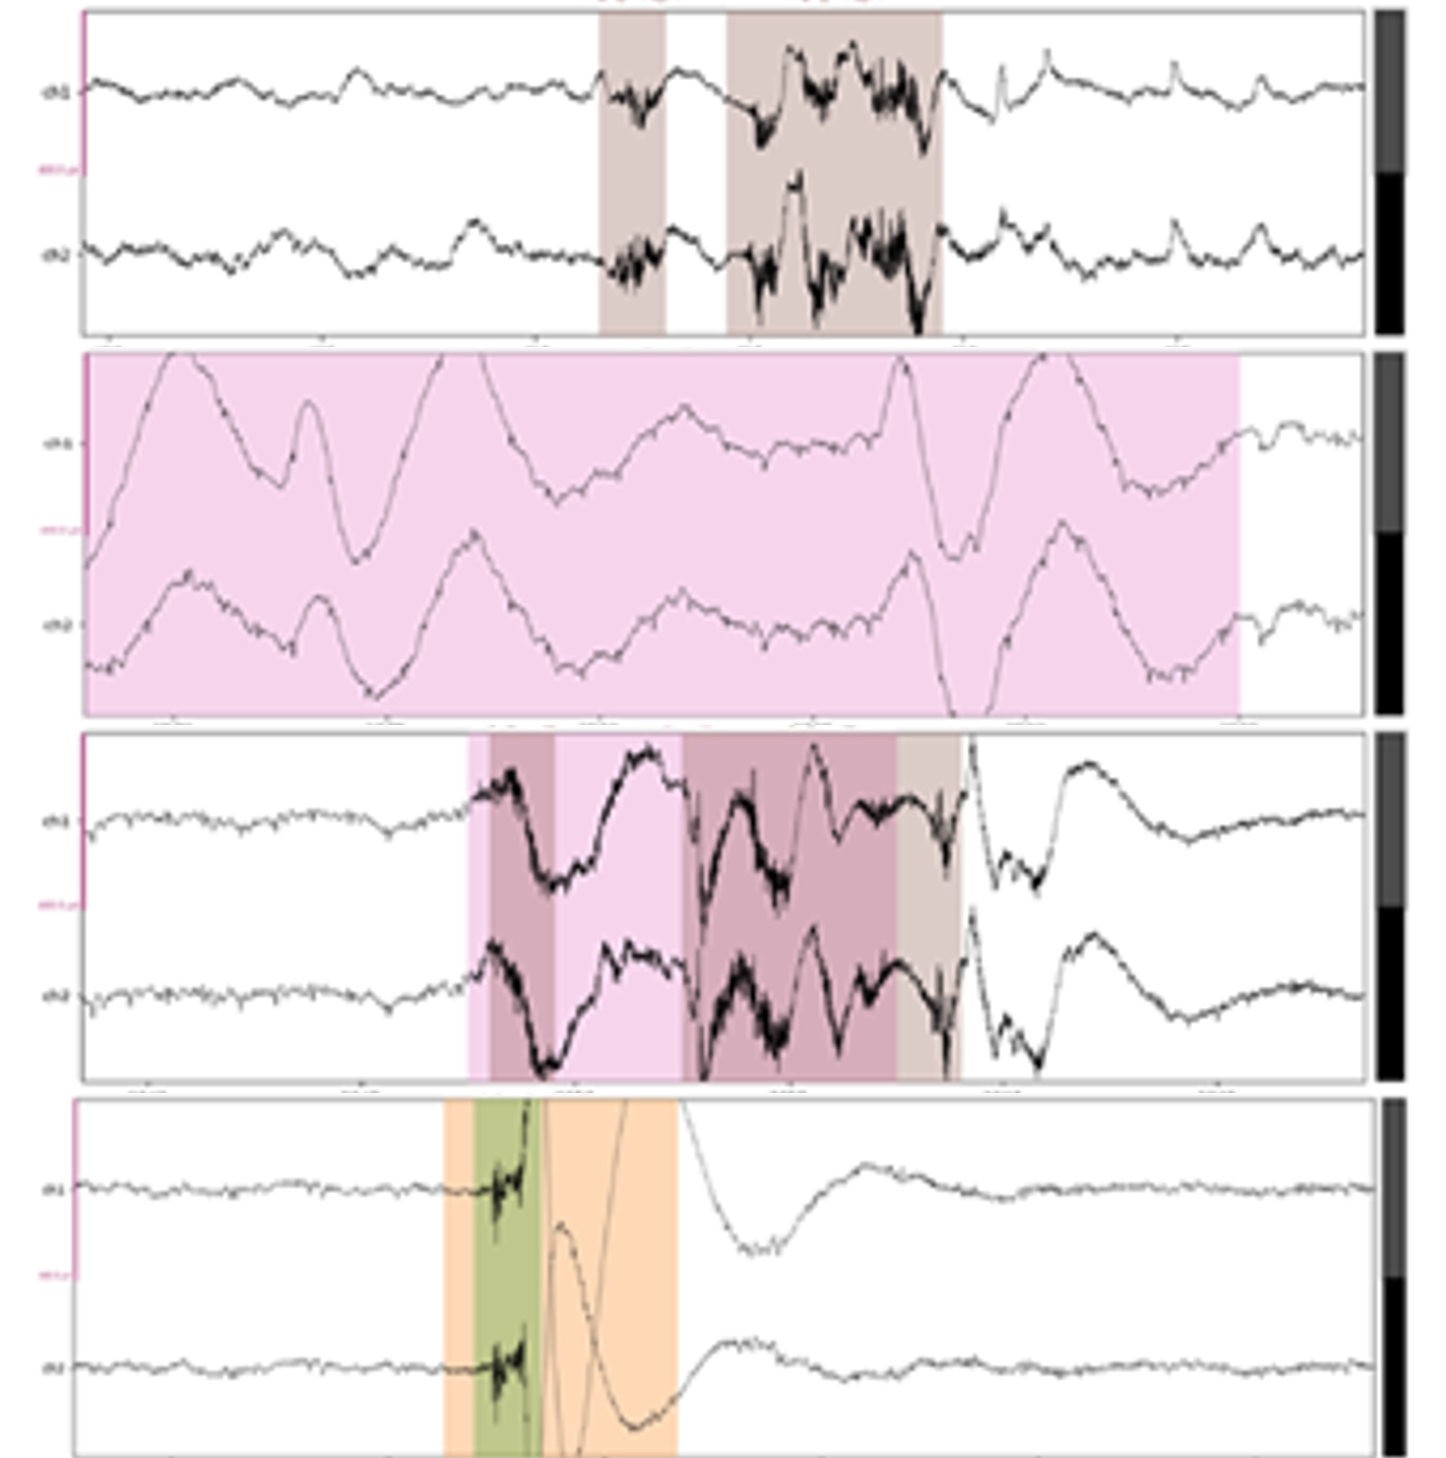
\includegraphics[width=0.95\columnwidth]{images/Fig1n.png}     
    \vspace{-0.1in}
    \caption{\label{fig:Fig1} Examples of the temporal visualization of EEG signals and coloring of noisy segments.}
    % \vskip -0.0in 
\end{figure}

In this figure, pink-colored areas are typical of low-frequency noise (0.2-4Hz), which is mainly due to perspiration originating from small drops of sweat produced by the skin glands, which cause changes in the electrical baseline of the electrodes. Brown-colored and green-colored areas are typical of high-frequency noise (30-45Hz) that may originate from electrical activity produced by the muscles when they are contracted, like, for example, muscle tension in the jaw or forehead that can take place when clenching or frowning, respectively. Orange-colored areas are typical of high-amplitude noise that may be due to temporary failures in contact between the EEG sensor and the scalp produced by touching the sensor or by spontaneous changes in electrode-skin contact.

In this analysis, EEG signals collected from a headband with two EEG channels synchronized with medical-grade EEG devices are considered. The recorded signal frequency for each channel of the headband is 128Hz. These signals are grouped into consecutive 30-second segments, and each segment is further annotated by three experts, into one of five sleep stages: Wake, N1, N2, N3, and REM. These stages correspond to specific brain activity patterns, such as slow eye movements, sleep spindles, and other characteristic waveforms. The goal of the current analysis is to detect the presence of noise, if any, at any of these segments. In total, 56 recordings were examined. Each recording refers to the EEG signals acquired by the headband of a user during a night-long sleep. These signals are grouped into 30-second consecutive segments.

As a ground-truth method to evaluate the results of the proposed noise estimation methods, the original estimation method used by the headband manufacturer is considered. This method consists of task-specific algorithms to automatically estimate noise and evaluate the overall quality of EEG signals, identifying the artifacts in recordings made using the wearable textile headband.

\subsection{Noise estimation methods training and set-up}

To train the machine learning models, the available recordings were
split into training (43 recordings), validation (3 recordings), and
testing subsets (10 recordings). Noise estimation is performed using
the test dataset. For the training configuration, we set the batch
size to 512 and trained the models for a maximum of 1000 epochs. To
prevent overfitting, we employ early stopping with patience of 30
epochs, meaning that if the validation loss does not improve for 30
consecutive epochs, training will stop. We set the learning rate to
1e-4 and use the Adam optimizer to adjust the model
weights. Additionally, we implement a ReduceLROnPlateau scheduler to
adjust the learning rate dynamically based on the validation loss. If
the validation loss plateaus, the scheduler reduces the learning rate
to help the model continue improving.

To process the input data, we split each 30-second segment of EEG
data---that consists of 7,680 EEG records per channel---into 32
smaller consecutive chunks, each consisting of a sequence of 240 EEG
records per channel. This structure allows the model to focus on both
the short and long-term temporal dependencies within the
data. Additionally, since the available dataset tends to overfit with
more complex models due to its low variability and extreme outliers,
simple architectures with only a few layers, e.g. a single attention
layer in the attention-based models, where considered. This approach
avoids unnecessary complexity, ensuring more stable training and
better generalization on the data.

Fig.~\ref{fig:Fig2} depicts the architecture of the Autoencoders developed for noise estimation on the examined test case. Input to the encoders is a sequence of 240 EEG records for both channels. Input data passes through an encoder and is compressed into a latent representation of size (1X8), where the first dimension represents a single compressed time step, and the second dimension represents eight learned features. The decoder then takes this compressed representation and attempts to reconstruct the original data, capturing both trends and amplitudes. 


\begin{figure}
    % \vskip -0.2in 
    \centering
    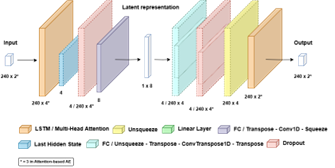
\includegraphics[width=0.95\columnwidth]{images/Fig2.png}     
    \vspace{-0.1in}
    \caption{\label{fig:Fig2} Architecture of the Autoencoders developed for noise estimation on the examined test case.}
    % \vskip -0.0in 
\end{figure}

The key difference between the two models lies in the method used for dimensionality reduction in the encoder and decoder: one uses fully connected (FC) layers, while the other uses convolutional layers. Both techniques aim to map the input data into a lower-dimensional latent space.

FC layers process the final hidden state of the LSTM (the last timestep in the sequence) as a single, comprehensive representation of the entire input sequence. This output is then projected into a lower-dimensional latent space through a linear transformation. While this approach is straightforward and computationally efficient, it assumes that all relevant temporal dependencies have already been captured in the LSTM's final output. As a result, it can struggle to retain fine-grained temporal details, especially for data like EEG signals, where localized patterns are crucial.

Conv1D layers operate directly on the sequence of hidden states output by the LSTM. By applying a kernel across the temporal dimension, they effectively extract localized patterns and dependencies across the sequence. The convolutional operation integrates information from multiple timesteps, creating a more nuanced and structured representation. After convolution, the output is reduced to a lower-dimensional latent space, where temporal features are preserved and compactly encoded. This method is particularly effective for sequential data like EEG, as it emphasizes localized temporal dynamics while reducing dimensionality.

Fig.~\ref{fig:Fig3} depicts the architecture of the Transformers developed for noise estimation on the examined test case. Input to the encoders is a sequence of 240 EEG records for both channels. 


\begin{figure}
    % \vskip -0.2in 
    \centering
    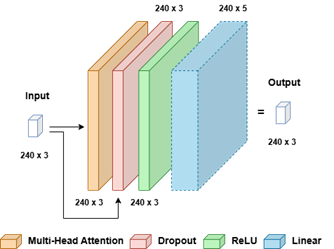
\includegraphics[width=0.95\columnwidth]{images/Fig3.png}     
    \vspace{-0.1in}
    \caption{\label{fig:Fig3} Architecture of the Transformers developed for noise estimation on the examined test case.}
    % \vskip -0.0in 
\end{figure}

The statistical methods are implemented using the Frouros\footnote{Documentation and source code are available at the official GitHub repository: \url{https://github.com/IFCA-Advanced-Computing/frouros}} open-source Python library designed for drift detection in machine learning systems.




%%%%%%%%%%%%
\section{EVALUATION AND RESULTS}
\label{sec:results}
%%%%%%%%%%%%

Table~\ref{tab2} presents the number of artifacts identified through
the estimation methodology employed by the headband manufacturer
across the ten recordings utilized to assess the anomaly detection
techniques. Specifically, it delineates the total count of 30-second
segments within which a minimum of one artifact is detected by the
headband manufacturer for each of the ten recordings, as recorded by
each EEG channel (designated as HB1 and HB2).

\begin{table}[bt]
\caption{Number of segments with artifacts on the testing recordings according to the headband manufacturer}
    \centering
    \renewcommand{\arraystretch}{1.3} % Adjust row height
    \begin{tabular}{|c|c|c|c|c|c|c|c|c|c|c|}
        \hline
        \textbf{Recording} & \textbf{1} & \textbf{2} & \textbf{3} & \textbf{4} & \textbf{5} & \textbf{6} & \textbf{7} & \textbf{8} & \textbf{9} & \textbf{10} \\
        \hline
        HB1 & 9 & 57 & 0 & 1 & 27 & 0 & 0 & 1 & 1 & 0 \\
        \hline
        HB2 & 9 & 56 & 0 & 0 & 26 & 151 & 0 & 1 & 1 & 0 \\
        \hline
    \end{tabular}
    \label{tab2}
\end{table}

The table illustrates that in 3 out of 10 recordings (3, 7, and 10), both channels detect no artifacts. In another 3 recordings (4, 8, and 9), only one segment is found contaminated with noise by both channels, except in recording 4, where the noise is identified solely by the HB1 channel. For the other two recordings (1 and 2), noisy segments are almost unanimously detected by both channels. Additionally, in recording 6, only the HB2 channel identifies noise in several segments, suggesting a potential issue with the corresponding sensor.



\begin{table*}[btp]
\centering
\caption{F-score, precision and recall on for different segment length.
  The F-score is calculated for $\beta=2$, emphasising recall over
  precision, as it approproate in out setting.
  Precision and recall, respectively, are given in parenthesis; When
  absent, it denoes that they are within three percentile points of
  the F2 score.
  Empty cells denote that the respective method did not mark any segment
  as noise, which implies that recall is 0\% and precision is undefined.}  
\label{tab:results}
\begin{sc}

\begin{subtable}[t]{\textwidth}
\centering
\caption{Evaluation on 30sec windows.}
\label{tab3}

\begin{tabular}{lp{\tbq}ccccccc}
      & \multicolumn{4}{c}{\textbf{HB1}} & \multicolumn{4}{c}{\textbf{HB2}} \\
\cmidrule(lr){2-5}\cmidrule(lr){6-9}
RecID &  A & B &  C & D &  A & B & C & D  \\
\cmidrule(lr){2-5}\cmidrule(lr){6-9}
LSTM  &    &\textbf{2\%}&   &   &\tbfs612          &\tbfs{7}{4}{4}&\tbfs{3}{4}{4} &     \\
C-LSTM&    &        &\tbmv{11}44&   &          &          &               &     \\
\cmidrule(lr){2-5}\cmidrule(lr){6-9}
AE\_err&    &        &   &   &                  &          &               &   \\
TP\_err  &    &        &   &   &                  &          &               &   \\
\cmidrule(lr){2-5}\cmidrule(lr){6-9}
AE\_att&    &\textbf{4\%}&    &   &\tbfs{20}11      &          &               &    \\
TP\_att  &    &\textbf{2\%}&    &   &\tbfs{13}{15}{15}&\tbfs{5}{14}{10}&\tbfs284&\tbfs1{11}{3}  \\
\cmidrule(lr){2-5}\cmidrule(lr){6-9}
PCA      &    &        &\tbmv{100}{85}{88}&\tbfs{100}{11}{14}
                              &\tbfs{41}{5}{6}&\tbfs{1}{4}{2}&\tbfs{24}{96}{60}&\tbfs{67}{22}{26} \\
MNE      &    &        &    &   &\tbfs{40}12      &          &               &     \\
\cmidrule(lr){2-5}\cmidrule(lr){6-9}
\end{tabular}
\end{subtable}

\vskip 1.5em
\begin{subtable}[t]{\textwidth}
\centering
\caption{Evaluation on 5min windows.}
\label{tab4}

\begin{tabular}{lp{\tbq}ccccccc}
          & \multicolumn{4}{c}{\textbf{HB1}} & \multicolumn{4}{c}{\textbf{HB2}} \\
\cmidrule(lr){2-5}\cmidrule(lr){6-9}
RecID &  A & \hskip -0.5cm B & \hskip -0.5cm C & D & A & B & C & D  \\
\cmidrule(lr){2-5}\cmidrule(lr){6-9}
LSTM	 &    &\tbmv6{18}{13}&       &   &\tbfs{12}{22}{19} &\tbms8{38}{22} &\tbms3{35}{11} &    \\
C-LSTM&    &             &\tbmv{10}{30}{21}& &\tbfs211  &               &               &\tbms1{11}4  \\
\cmidrule(lr){2-5}\cmidrule(lr){6-9}
AE\_err&    &\tbmv{27}{14}{16}&   &   &\tbfs{10}34       &               &               &    \\
TP\_err	 &    &             &       &   &                  &               &               &    \\
\cmidrule(lr){2-5}\cmidrule(lr){6-9}
AE\_att&    &\tbmv3{18}9  &\tbmv3{22}{10}&&\tbfs{18}67   &               &               &    \\
TP\_att	&    &\tbmv6{19}{14}&              & &\tbfs{14}{84}{42} &\tbms7{100}{26}&\tbms4{100}{16}&\tbms1{100}5   \\
\cmidrule(lr){2-5}\cmidrule(lr){6-9}
PCA	&    &              &\tbmv{77}{85}{83}&\tbfs{80}{89}{87} 
                                        &\tbfs{25}{21}{21}&\tbms3{27}{10}&\tbms{17}{96}{49}&\tbms{80}{89}{87}  \\
MNE	&    &              &       &\tbfs{82}{100}{96}
                                        &\tbfs{38}{13}{15}&   &           &\tbms{100}{11}{14}   \\
\cmidrule(lr){2-5}\cmidrule(lr){6-9}
\end{tabular}
\end{subtable}


\vskip 1.5em
\begin{subtable}[t]{\textwidth}
\centering
\caption{Evaluation on 10min windows.}
\label{tab5}

\begin{tabular}{lp{\tbq}ccccccc}
          & \multicolumn{4}{c}{\textbf{HB1}} & \multicolumn{4}{c}{\textbf{HB2}} \\
\cmidrule(lr){2-5}\cmidrule(lr){6-9}
RecID & A & B & \hskip -0.5cm C & D & A & B & C & D \\
\cmidrule(lr){2-5}\cmidrule(lr){6-9}
LSTM	  &   &\tbmv7{37}{19}&\tbmv2{11}5&   &\tbfs{12}{42}{28} &\tbfs7{64}{25} &\tbfs2{42}9    &    \\ 
C-LSTM &   &             &\tbmv{11}{67}{34}&&\tbfs111        &               &               & \tbfs5{100}{21} \\
\cmidrule(lr){2-5}\cmidrule(lr){6-9}
AE\_err &   &\tbmv{30}{32}{31}&            &   &\tbfs856          &               &               & \\
TP\_err	  &   &             &            &   &                  &               &               & \\
\cmidrule(lr){2-5}\cmidrule(lr){6-9}
AE\_att &   &\tbmv3{35}{12}&\tbmv7{89}{26}&&\tbfs{14}99       &               &               & \\
TP\_att	  &   &\tbmv7{39}{21}&\hskip -0.9cm \textbf{2\%}  &   &\tbfs{13}{90}{41} &\tbfs5{100}{22}&\tbfs3{100}{14}&\tbfs1{100}5\\
\cmidrule(lr){2-5}\cmidrule(lr){6-9}
PCA 	  &   &        &\hskip -1.1cm\tbfs{58}{85}{78}&\tbmv{82}{100}{96}
                                             &\tbfs{26}{40}{36} &\tbfs5{63}{19}&\tbfs{14}{96}{44}&\tbfs{82}{100}{96}\\
MNE	  &   &             &            &\tbmv{82}{100}{96}
                                             &\tbfs{35}{23}{25} &               & &\tbmv{82}{100}{96} \\
\cmidrule(lr){2-5}\cmidrule(lr){6-9}
\end{tabular}
\end{subtable}

\end{sc}
\end{table*}



Table~\ref{tab3} and Table~\ref{tab4} present the Precision and Recall metrics, respectively, for the evaluated methods across the seven test recordings (1, 2, 4, 5, 6, 8, and 9) where an artifact was detected by the manufacturer. All values are expressed as percentages.

The Precision metric in Table~\ref{tab3} denotes the percentage of
actual segments identified as having artifacts relative to the total
segments predicted to contain artifacts. However, this metric fails to
convey information regarding missed artifacts---specifically, those not
identified by the anomaly detection methodologies. This aspect is
quantified through the Recall metric (Table~\ref{tab4}), which
indicates the ratio of segments predicted to have artifacts against
the total number of actual segments containing artifacts. For
instance, the PCA method exhibits a precision of 100\% from the data
obtained during the HB1 test recording 1, yet it only achieves a
recall of 11.11\%. This discrepancy arises because the PCA method
successfully detected a singular artifact characterized by noise,
deemed a noisy artifact; thus, the precision remains at
100\%. However, it failed to identify the additional eight noisy
segments (refer to Table~\ref{tab2}), resulting in a significantly
reduced recall of approximately 11\%. Instances where there are empty
cells signify scenarios where the respective method did not identify
any artifacts. Consequently, precision cannot be ascertained, and
recall is recorded as 0\%.

In this application, our primary objective is to identify as many segments as possible that contain artifacts while allowing for some tolerance regarding detecting noisy segments. The principal aim should be to reduce the number of instances requiring the application of reliable yet non-automated anomaly detection methods. Consequently, the key performance metric to prioritize is Recall.

From the results presented in Table~\ref{tab3} and Table~\ref{tab4}, we conclude that all considered methods exhibited suboptimal performance. However, the PCA demonstrated relatively high recall values in two recordings. One plausible explanation for this observation could be the selected time-window of 30 seconds that defines the examined segment. The efficacy of anomaly detection methods in time series analysis may be significantly influenced by the length of the time series, as supported by existing literature \cite{Lee_2021}.

Due to this reasoning, we applied the selected methodologies to the same dataset while extending the segment duration from 30 seconds to 2, 5, and 10 minutes. Table~\ref{tab5}, Table~\ref{tab6}, and Table~\ref{tab7} illustrate the resulting recall values of the selected methods, respectively. 

One initial conclusion drawn is that across all methods analyzed, the detection of anomalies is significantly enhanced when the duration of the time-window assigned to each segment is increased. However, this improvement comes at the expense of broader time-windows during which the detected anomalies may actually occur---a consideration that necessitates careful evaluation. 

The primary conclusions are drawn through a comparative analysis of the performance of the evaluated methodologies. The introduced concept of utilizing attention mechanisms as a critical metric for anomaly detection appears to be promising. Across all segment durations (30 seconds, 2 minutes, 5 minutes, and 10 minutes), the Recall metrics for the AbAE\_att and TP\_att methods, which identify anomalies based on their attention matrix values, surpass those of their counterparts, AbAE\_err and TP\_err, which detect anomalies via reconstruction or prediction errors.

The performance of attention-based methods is generally comparable to, if not superior to, that of other state-of-the-art techniques, such as LSTM-AE and C-LSTM-AE. A similar conclusion can be derived from comparing the Recall values of the examined attention-based methods with those of baseline methods, including PCA and MNE. However, it is evident that the TP\_att method significantly outperforms the AbAE\_att method.



\section{CONCLUSIONS AND FUTURE WORK}
\label{sec:conc}
This paper investigates the innovative application of attention mechanisms within machine learning models, such as Autoencoders and Transformers, as pivotal indicators for anomaly detection in time-series datasets. Two methodologies, namely an Autoencoder and a Transformer, are examined, with their performances benchmarked against conventional techniques and other advanced machine-learning approaches. The efficacy of the proposed methodology is assessed utilizing electroencephalography (EEG) signals sourced from wearable sleep-monitoring devices, specifically measuring Precision and Recall against a manufacturer's established ground truth methodology. Findings indicate that attention-based approaches, particularly the Transformer Predictor, exhibit promising capabilities in identifying anomalies, particularly with extended time windows for analysis. The study concludes that attention mechanisms significantly enhance anomaly detection in streaming data environments.
The current study acts as a proof of concept, illustrating the potential of attention mechanisms as key-indicators of anomalies in time series data. Subsequent steps will entail exploring additional architectures beyond the AbAE\_att and TP\_att methods analyzed herein. Additionally, the investigation will focus on the performance parameters of attention-based techniques, such as the choice of time-window segments, to develop a task-agnostic approach for anomaly detection.



\ifnum\anon=0

%%%%%%%%%%%%
\section*{Acknowledgment}
%%%%%%%%%%%%

This research was co-funded by the European Union under GA no. 101135782 (MANOLO project). Views and opinions expressed are however those of the authors only and do not necessarily reflect those of the European Union or CNECT. Neither the European Union nor CNECT can be held responsible for them.
AWS resources were provided by the National Infrastructures for Research and Technology GRNET and funded by the EU Recovery and Resiliency Facility.

\fi

% \section*{References}

\bibliographystyle{IEEEtranDOI}
\bibliography{refs}

\end{document}
